\documentclass[tikz,convert={density=150,size=600,outext=.png}]{standalone}
\usetikzlibrary{shapes, calc, arrows, fit, positioning, decorations, patterns, decorations.pathreplacing, chains, snakes}

\begin{document}
  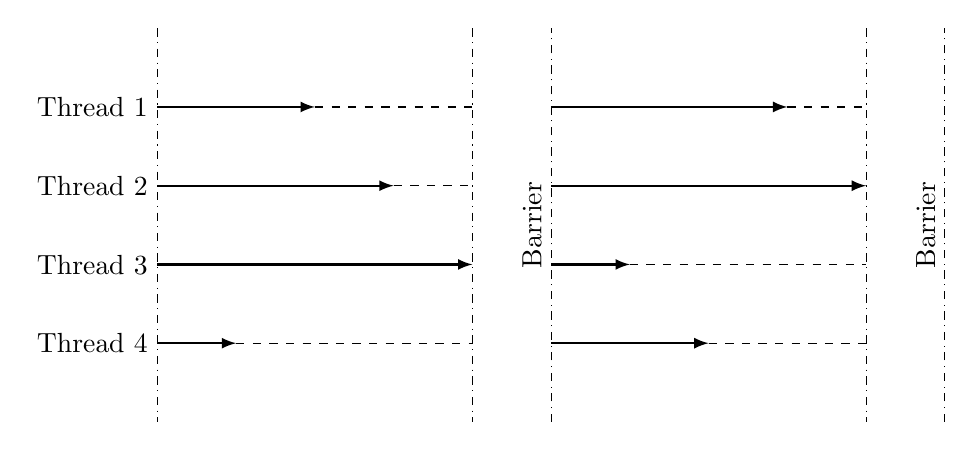
\begin{tikzpicture}[>=latex]
    \node[align=right, anchor=east] at (0, 0) {Thread 1};
    \node[align=right, anchor=east] at (0,-1) {Thread 2};
    \node[align=right, anchor=east] at (0,-2) {Thread 3};
    \node[align=right, anchor=east] at (0,-3) {Thread 4};

    \draw[->, thick] (0,0) -- (2, 0);
    \draw[-, dashed] (2,0) -- (4, 0);
    
    \draw[->, thick] (0,-1) -- (3, -1);
    \draw[-, dashed] (3,-1) -- (4, -1);

    \draw[->, thick] (0,-2) -- (4, -2);
    \draw[-, dashed] (4,-2) -- (4, -2);
    
    \draw[->, thick] (0,-3) -- (1, -3);
    \draw[-, dashed] (1,-3) -- (4, -3);
    
    \draw[->, thick] (0+5,0) -- (3+5, 0);
    \draw[-, dashed] (3+5,0) -- (4+5, 0);
    
    \draw[->, thick] (0+5,-1) -- (4+5, -1);
    \draw[-, dashed] (4+5,-1) -- (4+5, -1);

    \draw[->, thick] (0+5,-2) -- (1+5, -2);
    \draw[-, dashed] (1+5,-2) -- (4+5, -2);
    
    \draw[->, thick] (0+5,-3) -- (2+5, -3);
    \draw[-, dashed] (2+5,-3) -- (4+5, -3);

    \draw[dashdotted] (0,1) -- (0,-4);

    \draw[dashdotted] (4,1) -- (4,-4);
    \draw[dashdotted] (5,-4) -- (5,1) node[sloped,midway, above] {Barrier};
    
    \draw[dashdotted] (4+5,1) -- (4+5,-4);
    \draw[dashdotted] (5+5,-4) -- (5+5,1) node[sloped,midway, above] {Barrier};
  \end{tikzpicture}
\end{document}
